\documentclass[letterpaper]{article}
\DeclareSymbolFont{AMSb}{U}{msb}{m}{n}
\DeclareMathAlphabet{\mathbbm}{U}{bbm}{m}{n}

\title{Bifunctors}

\usepackage{amsmath,amssymb,amsthm,latexsym}
\usepackage[tiny,center,compact,sc]{titlesec}
\usepackage[cm]{fullpage}
\usepackage{bm}
\usepackage{tikz}
 \usetikzlibrary{arrows,calc,matrix,positioning,scopes}
\usepackage{textcomp}
\usepackage{mathtools}
\usepackage{hyperref}
% http://tex.stackexchange.com/questions/52410/how-to-use-the-command-autoref-to-implement-the-same-effect-when-use-the-comman
\def\equationautorefname~#1\null{(#1)\null}

\DeclarePairedDelimiterX\angles[1]{\langle}{\rangle}{#1}
\DeclarePairedDelimiterX\angbar[1]{\langlebar}{\ranglebar}{#1}
\DeclarePairedDelimiterX\paren[1]{(}{)}{#1}
\DeclarePairedDelimiterX\brak[1]{[}{]}{#1}
\DeclarePairedDelimiterX\abs[1]{\lvert}{\rvert}{#1}
\DeclarePairedDelimiterX\set[1]{\{}{\}}{#1}

% http://tex.stackexchange.com/questions/5502/how-to-get-a-mid-binary-relation-that-grows
\DeclareMathOperator{\mmid}{\mathrel{}\mathclose{}\delimsize|\mathopen{}\mathrel{}}

\newcommand{\defn}[1]{{\bf #1}}
\newcommand{\Hom}[3]{\textrm{Hom}_{#1}{\paren{#2,#3}}}

\renewcommand{\baselinestretch}{0.9}

\begin{document}

In the paper {\bf Functional Pearl: F for Functor} from ICPF '12, the
concept of a \defn{bifunctor} is introduced quickly and somewhat
confusingly.  Herein, as Neil Gaiman wrote in Good Omens,  ``the text will
be slowed down to allow the sleight of hand to be followed.''

\section{Bifunctors}

A \defn{bifunctor} is a two-argument object, here denoted $\textrm{---}
\otimes \textrm{---} \in \mathcal{E}^{\mathcal{C} \times \mathcal{D}}$,
which
%
\begin{itemize}
%
  \item Sends an object $C \times D \in \mathcal{C} \times \mathcal{D}$ to
  an object $C \otimes D \in \mathcal{E}$ and a morphism $f \times g \in
  \Hom{\mathcal{C} \times \mathcal{D}}{C \times D}{C' \times D'}$ to a
  morphism $f \otimes g \in \Hom{\mathcal{E}}{C \otimes D}{C' \otimes D'}$.
%
  \item Preserves identities ($id_C \otimes id_D = id_{C \otimes D}$) and
  composition: $(f' \circ f) \otimes (g' \circ g) = (f' \otimes g') \circ (f
  \otimes g)$.
%
  \item Has a $\mathcal{C}$-object-indexed collection of {\em functors}
  obtained by partial application on the left: a $L^\otimes_C = \paren{C
  \otimes \textrm{---}} \in \mathcal{E}^\mathcal{D}$ for each object $C \in
  \mathcal{C}$, and a $\mathcal{D}$-object-indexed collection from the
  right: a $R^\otimes_D \paren{\textrm{---} \otimes D} \in
  \mathcal{E}^\mathcal{C}$ for each object $D \in \mathcal{D}$.%
  %
  \footnote{Of course, there are also functor families indexed by arrows,
  which might be designated $\tilde{L}^\otimes_f = \paren{f \otimes
  \textrm{---}} \in \mathcal{E}^\mathcal{D}$ for each $f \in \mathcal{C}$.
  However, these bring no new degrees of freedom to the table, as
  $\tilde{L}^\otimes_f(D) = f \otimes D = R^\otimes_D f$ and
  $\tilde{L}^\otimes_f(g) = f \otimes g$.}
%
\end{itemize}

The question arises: if we have two collections of functors, $\set{
L^\otimes_C \in \mathcal{E}^\mathcal{D} \mmid C \in \mathcal{C}}$ and $\set{
R^\otimes_D \in \mathcal{E}^\mathcal{C} \mmid D \in \mathcal{D}}$, can we
stitch them together to make a bifunctor?  Looking at the object component
of our purported bifunctor $\otimes$, we see that $C \otimes D$ has two
possible definitions: $L^\otimes_C D$ and $R^\otimes_D C$.  These must be
equal in order for $\otimes$ to be well-defined:
%
\begin{equation}\label{eqn:objcoh} L^\otimes_C D = R^\otimes_D C \qquad
(\forall_{C \in \mathcal{C},D \in \mathcal{D}} . \text{diagram} \in
\mathcal{E} ) \end{equation}
%
What of the morphism map?  Given $f \in \Hom{\mathcal{C}}{C}{C'}$ and $g \in
\Hom{\mathcal{D}}{D}{D'}$, $f \otimes g$ expands in one of two ways, as
indicated by the following diagram.  These, too, must be equal for the
definition to make sense.  Note that \autoref{eqn:objcoh} allows us to label
the vertices of this diagram in an unambiguous, familiar syntax.

\begin{equation}\label{eqn:morcoh}
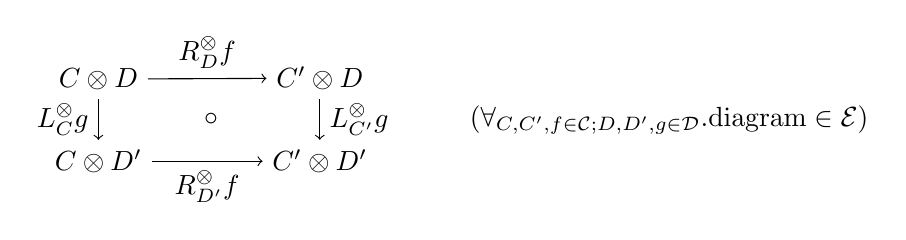
\begin{tikzpicture}
%
  \matrix[matrix of math nodes,column sep={80pt,between origins},
          row sep={30pt,between origins}] (m) {
%
    |[name=tl]| C \otimes D & |[name=tr]| C' \otimes D \\
%
    |[name=bl]| C \otimes D' & |[name=br]| C' \otimes D' \\
%
  } ;
%
  \node (m) {$\circ$} ;
%
  \node (m) [right=90pt] {$(\forall_{C,C',f \in \mathcal{C}; D,D',g \in \mathcal{D}} . \text{diagram} \in \mathcal{E})$} ;
%
  \draw [->] (tl) -- (tr) node [above,midway] {$R^\otimes_D f$} ;
  \draw [->] (tl) -- (bl) node [left,midway]  {$L^\otimes_C g$} ;
  \draw [->] (bl) -- (br) node [below,midway] {$R^\otimes_{D'} f$} ;
  \draw [->] (tr) -- (br) node [right,midway]  {$L^\otimes_{C'} g$} ;
%
\end{tikzpicture}
%
\end{equation}

Let us check that any $\set{L^\otimes_C \mmid C}$ and $\set{L^\otimes_D \mmid D}$ which
satisfy \autoref{eqn:objcoh} and \autoref{eqn:morcoh} in fact give rise to a
bifunctor.  We have our object and morphism maps and purported
partial-applications already, all that remains to be seen is preservation of
identity and composition.  Identity is easy:
%
\begin{align}
%
  id_C \otimes id_D
%
	&= \label{eqn:id1} L^\otimes_C id_D \circ R^\otimes_D id_C = id_{L^\otimes_C D} \circ id_{R^\otimes_D C} = id \\
%
	&= \label{eqn:id2} R^\otimes_D id_C \circ L^\otimes_C id_D = id_{R^\otimes_D C} \circ id_{L^\otimes_C D} = id
%
\end{align}
%
where \autoref{eqn:id1} is the right-then-down path and \autoref{eqn:id2} is the
down-then-right path in \autoref{eqn:morcoh}.  Note that we did {\em not}
need to assume anything to get this other than that $L^\otimes_C$ and $R^\otimes_D$ were
functors.  Composition unpacks a bit: $(f' \otimes g') \circ (f \otimes g)$
(for $f' \in \Hom{\mathcal{C}}{C'}{C''}$ and $g' \in
\Hom{\mathcal{D}}{D'}{D''}$ in addition to $f$ and $g$ as
above) has many possible meanings, each of which is a path through this
diagram:
%
\begin{equation}\label{eqn:comp}
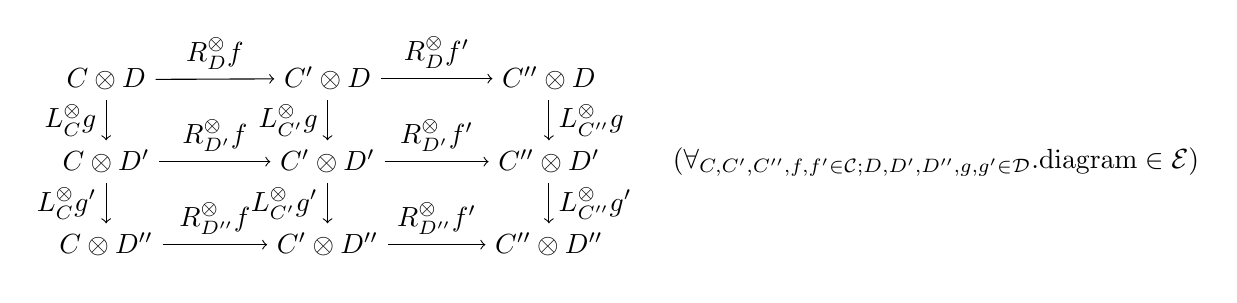
\begin{tikzpicture}
%
  \matrix[matrix of math nodes,column sep={80pt,between origins},
          row sep={30pt,between origins}] (m) {
%
    |[name=tl]| C \otimes D
  & |[name=tm]| C' \otimes D
  & |[name=tr]| C'' \otimes D \\
%
    |[name=ml]| C \otimes D'
  & |[name=mm]| C' \otimes D'
  & |[name=mr]| C'' \otimes D' \\
%
    |[name=bl]| C \otimes D''
  & |[name=bm]| C' \otimes D''
  & |[name=br]| C'' \otimes D'' \\
%
  } ;
%
  \node (m) [right=120pt] {$(\forall_{C,C',C'',f,f' \in \mathcal{C};
D,D',D'',g,g' \in \mathcal{D}} . \text{diagram} \in \mathcal{E})$} ;
%
  \draw [->] (tl) -- (tm) node [above,midway] {$R^\otimes_D f$} ;
  \draw [->] (tm) -- (tr) node [above,midway] {$R^\otimes_D f'$} ;
%
  \draw [->] (ml) -- (mm) node [above,midway] {$R^\otimes_{D'} f$} ;
  \draw [->] (mm) -- (mr) node [above,midway] {$R^\otimes_{D'} f'$} ;
% 
  \draw [->] (bl) -- (bm) node [above,midway] {$R^\otimes_{D''} f$} ;
  \draw [->] (bm) -- (br) node [above,midway] {$R^\otimes_{D''} f'$} ;
%
  \draw [->] (tl) -- (ml) node [left,midway]  {$L^\otimes_C g$} ;
  \draw [->] (tm) -- (mm) node [left,midway]  {$L^\otimes_{C'} g$} ;
  \draw [->] (tr) -- (mr) node [right,midway]  {$L^\otimes_{C''} g$} ;
%
  \draw [->] (ml) -- (bl) node [left,midway]  {$L^\otimes_C g'$} ;
  \draw [->] (mm) -- (bm) node [left,midway]  {$L^\otimes_{C'} g'$} ;
  \draw [->] (mr) -- (br) node [right,midway]  {$L^\otimes_{C''} g'$} ;
%
\end{tikzpicture}
%
\end{equation}

However, repeated application of \autoref{eqn:morcoh} lets us see that all
paths through this diagram are equal!  Moreover, the horizontal and vertical
paths correctly compose because each $L^\otimes_x$ and $R^\otimes_x$ are functors; that is,
along the top, for example: $R^\otimes_D f' \circ R^\otimes_D f = R^\otimes_D \paren{ f' \circ f }$.
We can see that the two possible expansions of $\paren{ f' \circ f } \otimes
\paren{ g' \circ g }$ (the two paths of \autoref{eqn:morcoh} with the
compositions in as the functions) are (respectively) equal to the two
outermost paths of \autoref{eqn:comp} and therefore to each other.

{\bf F for Functor} arrives at these conclusions in the reverse order.  That
is, it {\em defines} $f \otimes g$ as (in the notation of this document)
$L^\otimes_{C'} g \circ R^\otimes_{D} f$ (the top-right path of \autoref{eqn:morcoh}).  Then
it considers identity and composition, arriving (implicitly) at
\autoref{eqn:comp}.  ``Lambert'' computes the right-right-down-down and
right-down-right-down paths, in accordance with the bias of the definition
and concludes that the top-right rectangle of \autoref{eqn:comp} must
commute, thereby {\em deriving} \autoref{eqn:morcoh}.

\section{Natural Transformations}

We have used the exponential notation $\mathcal{E}^{\mathcal{C}}$ above
possibly somewhat prematurely.  While we could simply define functor
categories as discrete, let us instead not.  The objects of such a thing we
take to be functors from $\mathcal{C}$ to $\mathcal{E}$.  We will {\em
recover} the definition of morphisms in this category by considering a
particular bifunctor (later in the paper denoted $\star$) in
$\mathcal{E}^{\mathcal{E}^{\mathcal{C}} \times \mathcal{C}}$.  This
bifunctor's partial application views are $\set{L^\star_F \mmid F \in
\mathcal{E}^{\mathcal{C}}}$ (denoted $F \textrm{---}$ in the paper) and
$\set{R^\star_C \mmid C \in \mathcal{C}}$ (denoted $\textrm{---} A$ in the
paper).  $L^\star_F$ behaves as the functor $F$: it sends $C \in
\mathcal{C}$ to $FC \in \mathcal{E}$ and $f \in \Hom{\mathcal{C}}{C}{C'}$ to
$Ff \in \Hom{\mathcal{E}}{FC}{FC'}$.  This relies only on the objects of
$\mathcal{E}^\mathcal{C}$ and so is uninteresting.  What about $R^\star_C$?
If it is to be a functor, then:
%
\begin{itemize}
%
  \item The object component of $R^\star_C$ takes a functor $F \in
\mathcal{E}^{\mathcal{C}}$ to an object $F C \in \mathcal{E}$.
%
  \item The morphism component of $R^\star_C$ takes a morphism $\alpha \in
\Hom{\mathcal{E}^{\mathcal{C}}}{F}{G}$ to a morphism $R^\star_C \alpha \in
\Hom{\mathcal{E}}{R^\star_C F}{R^\star_C G} = \Hom{\mathcal{E}}{F C}{G C}$.
%
  \item It must map the identity morphism to an identity morphism:
$R^\star_C id_F = id_{F C}$.
%
  \item It must preserve composition: for any $\alpha \in
\Hom{\mathcal{E}^{\mathcal{C}}}{F}{G}$ and $\alpha' \in
\Hom{\mathcal{E}^{\mathcal{C}}}{G}{H}$, we must have that $R^\star_C
(\alpha' \circ \alpha) = (R^\star_C \alpha') \circ (R^\star_C \alpha)$.
%
  \item Furthermore, if $\star$ is to be a bifunctor, then
\autoref{eqn:morcoh} must hold (this diagram is over all $F,G \in
\mathcal{E}^\mathcal{C}$, $\alpha \in
\Hom{\mathcal{E}^{\mathcal{C}}}{F}{G}$, $C,C' \in \mathcal{C}$, and $f \in
\Hom{\mathcal{C}}{C}{C'}$; it ultimately takes place in $\mathcal{E}$):

\begin{equation}
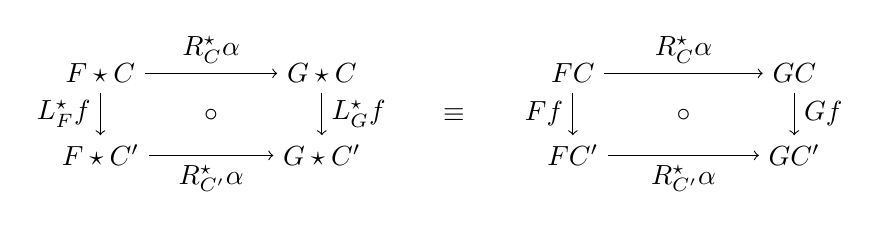
\begin{tikzpicture}
%
  \matrix (m) [matrix of math nodes,column sep={80pt,between origins},
          row sep={30pt,between origins}] {
%
    |[name=mtl]| F \star C & |[name=mtr]| G \star C \\
%
    |[name=mbl]| F \star C' & |[name=mbr]| G \star C' \\
%
  } ;
%
  \draw [->] (mtl) -- (mtr) node [above,midway] {$R^\star_C \alpha$} ;
  \draw [->] (mtl) -- (mbl) node [left,midway]  {$L^\star_F f$} ;
  \draw [->] (mbl) -- (mbr) node [below,midway] {$R^\star_{C'} \alpha$} ;
  \draw [->] (mtr) -- (mbr) node [right,midway]  {$L^\star_G f$} ;
%

  \node at (m) {$\circ$} ;

  \matrix (n) [matrix of math nodes,column sep={80pt,between origins},
          row sep={30pt,between origins},] at (6,0) {
%
    |[name=ntl]| F C & |[name=ntr]| G C \\
%
    |[name=nbl]| F C' & |[name=nbr]| G C' \\
%
  } ;

  \node at (n) {$\circ$} ;

  \draw [->] (ntl) -- (ntr) node [above,midway] {$R^\star_C \alpha$} ;
  \draw [->] (ntl) -- (nbl) node [left,midway]  {$F f$} ;
  \draw [->] (nbl) -- (nbr) node [below,midway] {$R^\star_{C'} \alpha$} ;
  \draw [->] (ntr) -- (nbr) node [right,midway]  {$G f$} ;

  \path (m) -- (n) node [midway] {$\equiv$} ;

\end{tikzpicture}
%
\end{equation}
%
\end{itemize}

Thus we can see that {\em if $\mathcal{E}^\mathcal{C}$ is to be a category}
whose objects are functors and {\em if $\star$ is to be a bifunctor}, then
{\em the morphisms} $\mathcal{E}^\mathcal{C}$ must exist in correspondence
with any subset of the natural transformations in $\mathcal{E}$ which
includes the identity natural transformations of every functor in
$\mathcal{E}^{\mathcal{C}}$.  We are free to pick the maximal such category,
and (abusively) suppress the $R^\star$ notation, to claim that the morphisms
of $\mathcal{E}^{\mathcal{C}}$ {\em are} the natural transformations between
its functors.

\subsection{Composition of Nat. Trans}

This has always confused me, so here's an excellent opportunity to expando
the notation and hopefully make some things clearer.  Frustratingly, {\bf F
for Functor} uses $\cdot$ for ordinary composition (while standard notation
is $\circ$) and $\circ$ for another composition operator on nat. trans.
Here we use $\circ$ and $\bigcirc$.

We begin by considering a bifunctor which composes functors, called
$\textrm{---} \bigcirc \textrm{---}$.  It is an object of the (visually
intimidating) category
$\paren{\mathcal{E}^\mathcal{C}}^{\mathcal{E}^{\mathcal{D}} \times
\mathcal{D}^{\mathcal{C}}}$.  Adopting and extending the paper's naming
scheme, let $G,K,Q \in \mathcal{E}^{\mathcal{D}}$; $\alpha,\alpha' \in
\Hom{\mathcal{E}^{\mathcal{D}}}{G}{K}$; $F,H,P \in
\mathcal{D}^{\mathcal{C}}$; $\beta,\beta' \in
\Hom{\mathcal{D}^{\mathcal{C}}}{F}{H}$; $C,C' \in \mathcal{C}$; $f \in
\Hom{\mathcal{C}}{C}{C'}$; $D,D' \in \mathcal{D}$; and $g \in
\Hom{\mathcal{D}}{D}{D'}$.  First note, as the paper does, that we have that
$G \bigcirc F \in \mathcal{E}^{\mathcal{C}}$ and $\beta \bigcirc \alpha \in
\Hom{\mathcal{E}^{\mathcal{C}}}{G \bigcirc F}{K \bigcirc H}$. (These hold
under exchange of similarly-quantified names, of course.)

If we just write down everything we know (a popular technique for earning
sympathy on exams), we first get these two ``vertical composition''
diagrams (in $\mathcal{D}$ and $\mathcal{E}$, respectively):
\begin{equation}
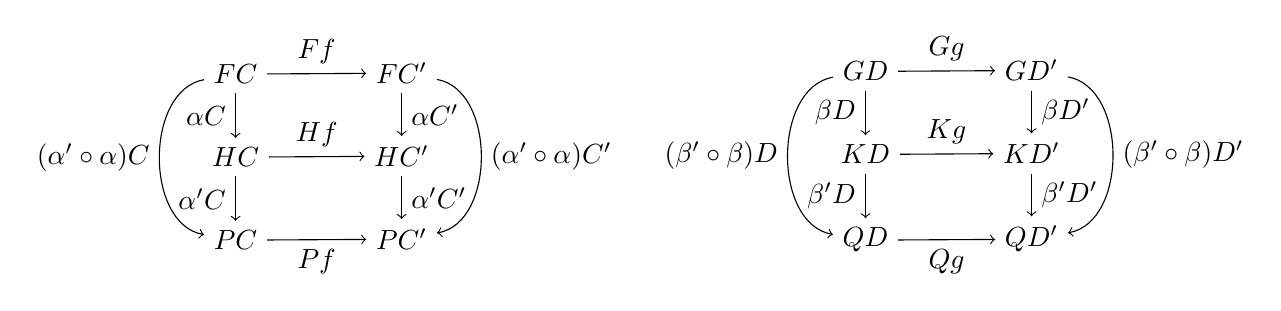
\begin{tikzpicture}
  \matrix[matrix of math nodes,column sep={60pt,between origins},
          row sep={30pt,between origins}] (m) {
%
  |[name=mtl]| F C & |[name=mbl]| F C' \\
  |[name=mtm]| H C & |[name=mbm]| H C' \\
  |[name=mtr]| P C & |[name=mbr]| P C' \\
%
  } ;
%
  \draw [->] (mtl) -- (mtm) node [left,midway] {$\alpha C$} ;
  \draw [->] (mtm) -- (mtr) node [left,midway] {$\alpha' C$} ;
%
  \draw [->] (mbl) -- (mbm) node [right,midway] {$\alpha C'$} ;
  \draw [->] (mbm) -- (mbr) node [right,midway] {$\alpha' C'$} ;
%
  \draw [->] (mtl) -- (mbl) node [above,midway]  {$F f$} ;
  \draw [->] (mtm) -- (mbm) node [above,midway]  {$H f$} ;
  \draw [->] (mtr) -- (mbr) node [below,midway] {$P f$} ;

  \draw [->] (mtl) to[bend right=80] node [left] {$(\alpha' \circ \alpha) C$} (mtr) ;
  \draw [->] (mbl) to[bend left=80] node [right] {$(\alpha' \circ \alpha) C'$} (mbr) ;
%

  \matrix[matrix of math nodes,column sep={60pt,between origins},
          row sep={30pt,between origins}] (l) at (8,0) {
%
  |[name=ltl]| G D & |[name=lbl]| G D' \\
  |[name=ltm]| K D & |[name=lbm]| K D' \\
  |[name=ltr]| Q D & |[name=lbr]| Q D' \\
%
  } ;
%
  \draw [->] (ltl) -- (ltm) node [left,midway] {$\beta D$} ;
  \draw [->] (ltm) -- (ltr) node [left,midway] {$\beta' D$} ;
%
  \draw [->] (lbl) -- (lbm) node [right,midway] {$\beta D'$} ;
  \draw [->] (lbm) -- (lbr) node [right,midway] {$\beta' D'$} ;
%
  \draw [->] (ltl) -- (lbl) node [above,midway]  {$G g$} ;
  \draw [->] (ltm) -- (lbm) node [above,midway]  {$K g$} ;
  \draw [->] (ltr) -- (lbr) node [below,midway] {$Q g$} ;
%

  \draw [->] (ltl) to[bend right=80] node [left] {$(\beta' \circ \beta) D$} (ltr) ;
  \draw [->] (lbl) to[bend left=80] node [right] {$(\beta' \circ \beta) D'$} (lbr) ;

\end{tikzpicture}
%
\end{equation}
%
We also get this ``horizontal composition'' diagram in $\mathcal{E}$:
%
\begin{equation}
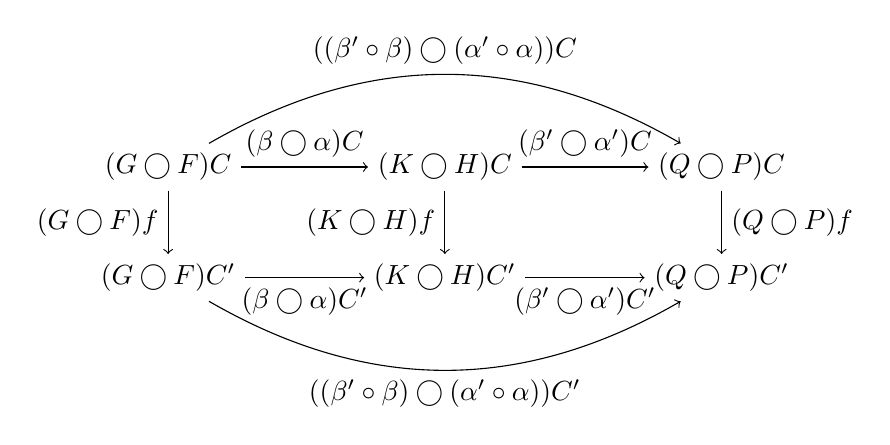
\begin{tikzpicture}

  \matrix[matrix of math nodes,column sep={100pt,between origins},
          row sep={40pt,between origins}] (m) {
%
    |[name=mtl]| (G \bigcirc F) C 
  & |[name=mtm]| (K \bigcirc H) C
  & |[name=mtr]| (Q \bigcirc P) C \\
%
    |[name=mbl]| (G \bigcirc F) C'
  & |[name=mbm]| (K \bigcirc H) C'
  & |[name=mbr]| (Q \bigcirc P) C' \\
%
  } ;
%
  \draw [->] (mtl) -- (mtm) node [above,midway] {$(\beta \bigcirc \alpha) C$} ;
  \draw [->] (mtm) -- (mtr) node [above,midway] {$(\beta' \bigcirc \alpha') C$} ;
%
  \draw [->] (mbl) -- (mbm) node [below,midway] {$(\beta \bigcirc \alpha) C'$} ;
  \draw [->] (mbm) -- (mbr) node [below,midway] {$(\beta' \bigcirc \alpha') C'$} ;
%
  \draw [->] (mtl) -- (mbl) node [left,midway]  {$(G \bigcirc F) f$} ;
  \draw [->] (mtm) -- (mbm) node [left,midway]  {$(K \bigcirc H) f$} ;
  \draw [->] (mtr) -- (mbr) node [right,midway] {$(Q \bigcirc P) f$} ;
%
  \draw [->] (mtl) to[bend left] node [above] {$((\beta' \circ \beta) \bigcirc (\alpha' \circ \alpha)) C$} (mtr) ;

  \draw [->] (mbl) to[bend right] node [below] {$((\beta' \circ \beta) \bigcirc (\alpha' \circ \alpha)) C'$} (mbr) ;

\end{tikzpicture}
%
\end{equation}
The rectangles commute by definition of natural transformations while the
upper and lower faces commute by bifunctorality of $\bigcirc$ (namely, that it
preserves composition).


\end{document}
